\chapter{Anexos}
\label{ch:Anexos}

A continuación se describen todas las opciones de grados y títulos disponibles en la memoria.

\section{Imagenes}

\begin{figure}[H]
    \centering
    \caption{\label{fig:rectaPCA} Ejemplo de recta que disminuye las distancias de los puntos a ella.}
    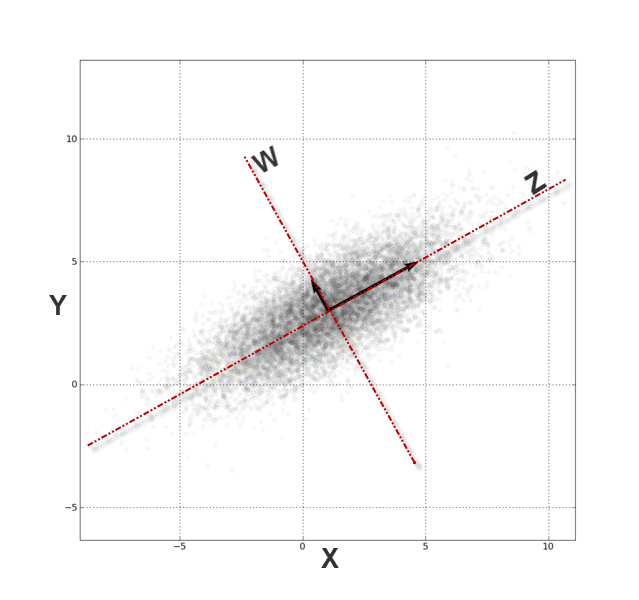
\includegraphics[width=0.5\textwidth]{figures/graficaRectaPCA.png}
\end{figure}
\begin{center}
    [Fuente:\href{https://cutt.ly/AmJ3I9M}{https://cutt.ly/AmJ3I9M}] \cite{Mohamed}
\end{center}

\begin{figure}[H]
    \centering
    \caption{\label{fig:representacionPCA} Ejemplo de  representación gráfica PCA.}
    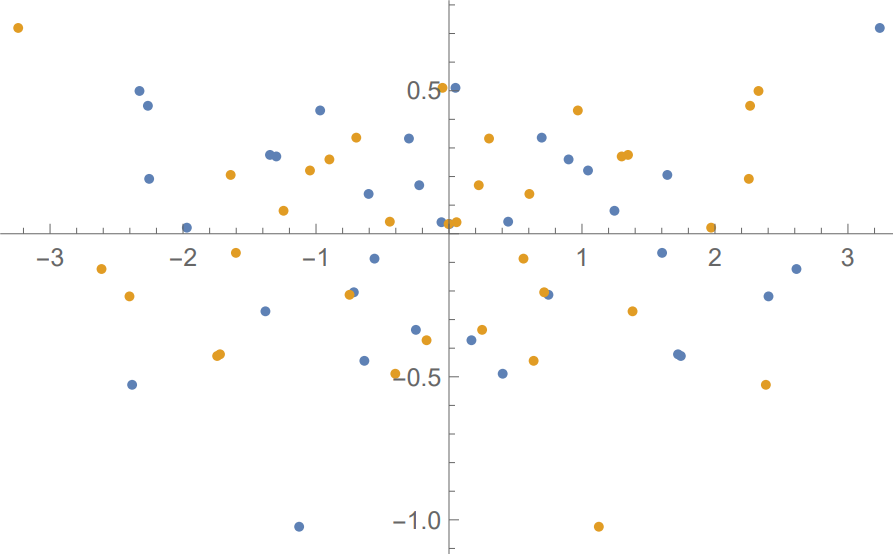
\includegraphics[width=0.5\textwidth]{figures/Dplot.png}
\end{figure}
\begin{center}
    [Fuente: Elaboración propia en Mathematica] 
\end{center}

\begin{figure}[H]
    \centering
    \caption{\label{fig:representacion3D} Ejemplo de  representación gráfica 3D PCA.}
    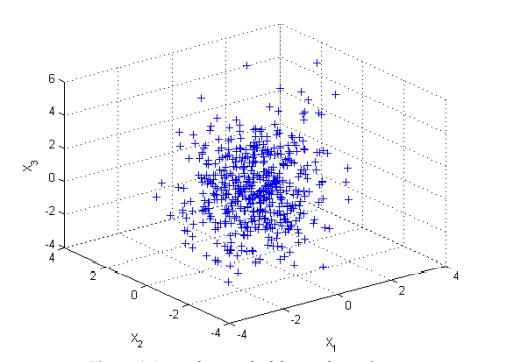
\includegraphics[width=0.5\textwidth]{figures/grafico3D.png}
\end{figure}
\begin{center}
    [Fuente: Analisis de componentes principales: Versiones dispersas y robustas al ruido impulsivo]\cite{andresSanchesMangas} 
\end{center}


\section{Cuadros}
\newpage


\begin{table}[H]
    \centering
    \begin{tabular}{|c|c|c|c|c|c|c|c|c|}
\hline
\textbf{ID} & \textbf{T1} & \textbf{T2} & \textbf{T3} & \textbf{Exp} & \textbf{P1} & \textbf{P2} & \textbf{Proy} & \textbf{Nota Final} \\ \hline
1           & 93          & 90          & 100         & 100          & 21.27       & 40          & 50            & 53.90083333         \\ \hline
2           & 96          & 95          & 100         & 100          & 55.31       & 73.3        & 90            & 79.4025             \\ \hline
3           & 88          & 70          & 90          & 90           & 0           & 30          & 80            & 48.66666667         \\ \hline
4           & 15          & 25          & 0           & 0            & 21.27       & 0           & 30            & 14.65083333         \\ \hline
5           & 88          & 70          & 95          & 100          & 78.72       & 63.3        & 80            & 77.58833333         \\ \hline
6           & 78          & 70          & 0           & 0            & 51.06       & 36.6        & 45            & 43.24833333         \\ \hline
7           & 93          & 90          & 100         & 100          & 43.42       & 73.3        & 50            & 67.76333333         \\ \hline
8           & 93          & 90          & 60          & 0            & 0           & 26.6        & 50            & 36.9                \\ \hline
9           & 63          & 100         & 0           & 70           & 27.65       & 46.6        & 85            & 52.64583333         \\ \hline
10          & 63          & 100         & 0           & 0            & 0           & 0           & 85            & 30.58333333         \\ \hline
11          & 0           & 0           & 0           & 0            & 0           & 0           & 0             & 0                   \\ \hline
12          & 88          & 70          & 95          & 80           & 85.1        & 76.6        & 80            & 81.50833333         \\ \hline
13          & 53          & 0           & 0           & 0            & 23.4        & 0           & 0             & 10.26666667         \\ \hline
14          & 58          & 0           & 100         & 90           & 36.17       & 0           & 50            & 36.70916667         \\ \hline
15          & 58          & 0           & 0           & 90           & 0           & 0           & 0             & 9.333333333         \\ \hline
16          & 78          & 70          & 90          & 100          & 68.08       & 31.6        & 45            & 58.75333333         \\ \hline
17          & 0           & 45          & 0           & 0            & 0           & 0           & 0             & 3.75                \\ \hline
18          & 78          & 70          & 90          & 85           & 65.95       & 0           & 45            & 49.57083333         \\ \hline
19          & 68          & 65          & 75          & 100          & 14.89       & 0           & 80            & 42.05583333         \\ \hline
20          & 93          & 85          & 0           & 0            & 29.78       & 0           & 0             & 22.27833333         \\ \hline
21          & 78          & 70          & 90          & 85           & 63.82       & 46.6        & 45            & 60.68833333         \\ \hline
22          & 88          & 70          & 90          & 80           & 82.97       & 80          & 80            & 81.40916667         \\ \hline
23          & 93          & 85          & 0           & 0            & 27.65       & 0           & 50            & 31.74583333         \\ \hline
24          & 96          & 95          & 100         & 100          & 53.19       & 50          & 90            & 73.0475             \\ \hline
25          & 88          & 70          & 90          & 90           & 46.8        & 66.6        & 80            & 69.51666667         \\ \hline
26          & 93          & 90          & 100         & 100          & 65.95       & 66.6        & 50            & 71.72083333         \\ \hline
27          & 78          & 70          & 0           & 100          & 19.14       & 0           & 45            & 31.11833333         \\ \hline
28          & 58          & 10          & 85          & 90           & 27.65       & 30          & 40            & 39.6625             \\ \hline
29          & 63          & 100         & 0           & 50           & 40.42       & 0           & 85            & 43.18833333         \\ \hline
30          & 0           & 0           & 0           & 0            & 19.14       & 0           & 0             & 4.785               \\ \hline
31          & 93          & 85          & 0           & 0            & 8.51        & 0           & 0             & 16.96083333         \\ \hline
32          & 93          & 85          & 100         & 100          & 63.82       & 63.3        & 85            & 76.94666667         \\ \hline
33          & 93          & 85          & 100         & 100          & 42.55       & 36.6        & 50            & 57.95416667         \\ \hline
34          & 58          & 0           & 0           & 0            & 19.14       & 0           & 0             & 9.618333333         \\ \hline
35          & 63          & 100         & 0           & 100          & 29.78       & 20          & 85            & 48.02833333         \\ \hline
36          & 15          & 25          & 0           & 100          & 38.29       & 0           & 30            & 23.90583333         \\ \hline
37          & 0           & 25          & 0           & 0            & 8.51        & 0           & 0             & 4.210833333         \\ \hline
38          & 96          & 95          & 100         & 100          & 0           & 60          & 90            & 62.25               \\ \hline
39          & 68          & 65          & 90          & 100          & 29.78       & 26.6        & 80            & 53.67833333         \\ \hline
40          & 96          & 95          & 100         & 100          & 27.65       & 80          & 90            & 74.1625             \\ \hline
41          & 96          & 95          & 100         & 100          & 74.46       & 56.6        & 90            & 80.015              \\ \hline
42          & 68          & 65          & 75          & 100          & 40.42       & 50          & 80            & 60.93833333         \\ \hline
43          & 15          & 25          & 0           & 100          & 38.29       & 0           & 30            & 23.90583333         \\ \hline
44          & 68          & 65          & 90          & 100          & 34.65       & 40          & 80            & 58.24583333         \\ \hline
\end{tabular}
    \caption{Notas del curso MA0321 del año 2020}
    \label{tab:notas}
\end{table}


